\documentclass{article}
\usepackage{amsmath}
\usepackage{amssymb}
\usepackage{hyperref} % For clickable table of contents
\usepackage{tikz}
\usetikzlibrary{arrows.meta, positioning}

\title{CPSC 354 Report}
\author{Drew Floyd}
\date{}

\begin{document}

\maketitle
\tableofcontents
\newpage

\section{The MU-Puzzle}

MI $\rightarrow$ MU

\textbf{Rule 1:} If you possess a string whose last letter is \texttt{I}, add \texttt{U}.

\textbf{Rule 2:} Suppose you have \texttt{Mx}, you may add \texttt{Mxx}.

\textbf{Rule 3:} If \texttt{III} occurs in one of the strings, you may make a new string with \texttt{U} in place of \texttt{III}.

\textbf{Rule 4:} If \texttt{UU}, you can drop it.

\vspace{1em}

MI \\
MII $\; Mxx$ \\
MIIII $\; Mxx$ \\
MIIIIIIII $\; Mxx$ \\
MUIIU $\; MIU$ \\
$\varnothing$

\vspace{1em}

MI $\; \rightarrow$ use $Mxx$ rule $\infty$ times \\
MIIII... \\

No matter what Rule you use you will never be able to get 0 Mod3, because I will always be 1 mod 3 or 2 mod 3

\vspace{1em}

\texttt{MUUU} \\
\texttt{MIII}

\vspace{1em}

\textbf{Rule 1} does not affect \# of I's. \\
\textbf{Rule 2} does not give 0 mod 3. \\
\textbf{Rule 3} does not solve the problem as removing 3 I's does not change the output of mod3. \\
\textbf{Rule 4} does not change the \# of I's. \\

We can never get rid of all of the I's, 0 mod 3 is not possible. Thus you cannot get MU from MI.

\newpage

\section{Rewriting Assignment}

\begin{enumerate}
    \item $A = \{ \}$ \\
    \hspace*{1em} $R = \{ \}$

    \begin{center}
        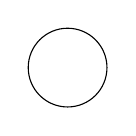
\begin{tikzpicture}
        \node[circle, draw, minimum size=1cm] (a) {};
        % Ensure the node is properly placed and visible
        \path (a) ++(0,0);
        \end{tikzpicture}
        \end{center}
    This diagram is terminating because there are no infinite loops, confluent because all paths lead to the same result, and has a unique normal form as there is only one final state.

    \item $A = \{ a \}$ \\
    \hspace*{1em} $R = \{ \}$

    \begin{center}
    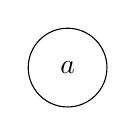
\begin{tikzpicture}
        \node[circle, draw, minimum size=1cm] (a) {$a$};
    \end{tikzpicture}
    \end{center}
    This diagram is terminating because there are no infinite loops, confluent because all paths lead to the same result, and has a unique normal form as there is only one final state.

    \item $A = \{ a \}$ \\
    \hspace*{1em} $R = \{ (a,a) \}$

    \begin{center}
    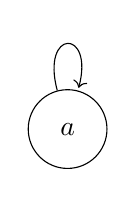
\begin{tikzpicture}
        \node[circle, draw, minimum size=1cm] (a) {$a$};
        \draw[->] (a) edge[loop above] (a);
    \end{tikzpicture}
    \end{center}
    This diagram is not terminating due to the presence of infinite loops, confluent because all paths merge, but does not have a unique normal form as multiple results are possible.

    \item $A = \{ a, b, c \}$ \\
    \hspace*{1em} $R = \{ (a,b), (a,b) \}$

    \begin{center}
    \begin{tikzpicture}
        \node[circle, draw, minimum size=1cm] (a) {$a$};
        \node[right=2cm of a, circle, draw, minimum size=1cm] (b) {$b$};
        \node[below=2cm of a, circle, draw, minimum size=1cm] (c) {$c$};
        \draw[->] (a) -- (b);
        \draw[->] (a) -- (c);
    \end{tikzpicture}
    \end{center}
    This diagram is terminating as there are no infinite loops, not confluent because paths diverge, and does not have a unique normal form due to multiple end states.

    \item $A = \{ a, b \}$ \\
    \hspace*{1em} $R = \{ (a,a), (a,b) \}$

    \begin{center}
    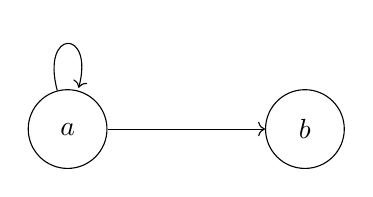
\begin{tikzpicture}
        \node[circle, draw, minimum size=1cm] (a) {$a$};
        \node[right=2cm of a, circle, draw, minimum size=1cm] (b) {$b$};
        \draw[->] (a) -- (b);
        \draw[->] (a) edge[loop above] (a);
    \end{tikzpicture}
    \end{center}
    This diagram is not terminating due to the presence of infinite loops, not confluent because paths diverge, and has a unique normal form due to having a single end state on b.

    \item $A = \{ a, b, c \}$ \\
    \hspace*{1em} $R = \{ (a,b), (b,b), (a,c) \}$
%  #6
    \begin{center}
    \begin{tikzpicture}
        \node[circle, draw, minimum size=1cm] (a) {$a$};
        \node[right=2cm of a, circle, draw, minimum size=1cm] (b) {$b$};
        \node[below=2cm of a, circle, draw, minimum size=1cm] (c) {$c$};
        \draw[->] (a) -- (b);
        \draw[->] (a) -- (c);
        \draw[->] (b) edge[loop above] (b);
    \end{tikzpicture}
    \end{center}
    This diagram is not terminating due to the presence of infinite loops, not confluent because paths diverge, and has a unique normal form due to having a single end state on c.

    \item $A = \{ a, b, c \}$ \\
    \hspace*{1em} $R = \{ (a,b), (b,b), (a,c), (c,c) \}$

    \begin{center}
    \begin{tikzpicture}
        \node[circle, draw, minimum size=1cm] (a) {$a$};
        \node[right=2cm of a, circle, draw, minimum size=1cm] (b) {$b$};
        \node[below=2cm of a, circle, draw, minimum size=1cm] (c) {$c$};
        \draw[->] (b) edge[loop above] (b);
        \draw[->] (c) edge[loop below] (c);
        \draw[->] (a) -- (b);
        \draw[->] (a) -- (c);
    \end{tikzpicture}
    \end{center}
    This diagram is not terminating due to the presence of infinite loops, not confluent because paths diverge, and does not have a unique normal form due to no end states.
\end{enumerate}

\section*{Properties}
\begin{tabular}{c c c c}
     & T & C & N \\ \hline
    1. & $\checkmark$ & $\checkmark$ & $\checkmark$ \\
    2. & $\checkmark$ & $\checkmark$ & $\checkmark$ \\
    3. & $\times$ & $\checkmark$ & $\times$ \\
    4. & $\checkmark$ & $\times$ & $\times$ \\
    5. & $\times$ & $\times$ & $\checkmark$ \\
    6. & $\times$ & $\times$ & $\checkmark$ \\
    7. & $\times$ & $\times$ & $\times$ \\
\end{tabular}

\vspace{1em}
\noindent Terminating, Confluent, Unique Normal Form

\end{document}
